\chapter{Resultados}\label{cap4} % con la palabra capitulo
\graphicspath{{./graficas}}
%\addcontentsline{toc}{chapter}{Capítulo 2: Marco Teórico} % si queremos que aparezca en el Í­ndice
%\markboth{Capítulo 2: Marco Teórico}{Capítulo 2: Marco Teórico} % encabezado
\linespread{1.3}
En la Figura \ref{fig:graf} se muestra un ejemplo de una grafica añadida en formado .pdf (puede utilizarse formato .jpg, .png o directamente desde software graficador en formato .tex)
\begin{figure}[hbtp]
\centering
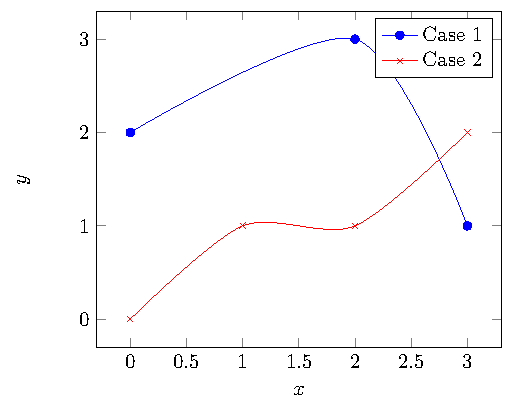
\includegraphics[scale=1]{/pg.pdf}
\caption{ejemplo de gráfica.}
\label{fig:graf}
\end{figure}
\clearpage%